\subsection{HBV-96 (model ID: 37)}
The HBV-96 model (fig.~\ref{fig:37_schematic}) was originally developed for use in Sweden, but has been widely applied beyond its original region \citep{Lindstrom1997}. It can account for different land types (forest, open ground, lakes) but that distinction has been removed here. Correction factors for climate inputs have also been removed. It has 5 stores and 15 parameters ($TT$, $TTI$, $CFR$, $CFMAX$, $TTM$, $WHC$, $CFLUX$, $FC$, $LP$, $\beta$, $K_0$, $\alpha$, $c$, $K_1$ and $MAXBAS$) parameters. The model aims to represent:

\begin{itemizecompact}
\item Snow accumulation, melt and refreezing;
\item Infiltration and capillary flow to, and evaporation from, soil moisture;
\item A non-linear storage-runoff relationship from the upper runoff-generating zone;
\item A linear storage-runoff relationship from the lower runoff-generating zone.
\end{itemizecompact}

\subsubsection{File names}
\begin{tabular}{@{}ll}
Model: &m\_37\_hbv\_15p\_5s \\
Parameter ranges: &m\_37\_hbv\_15p\_5s\_parameter\_ ranges \\
\end{tabular}

% Equations
\subsubsection{Model equations}

% Model layout figure
{ 																	% This ensures it doesn't warp text further down
\begin{wrapfigure}{l}{5cm}
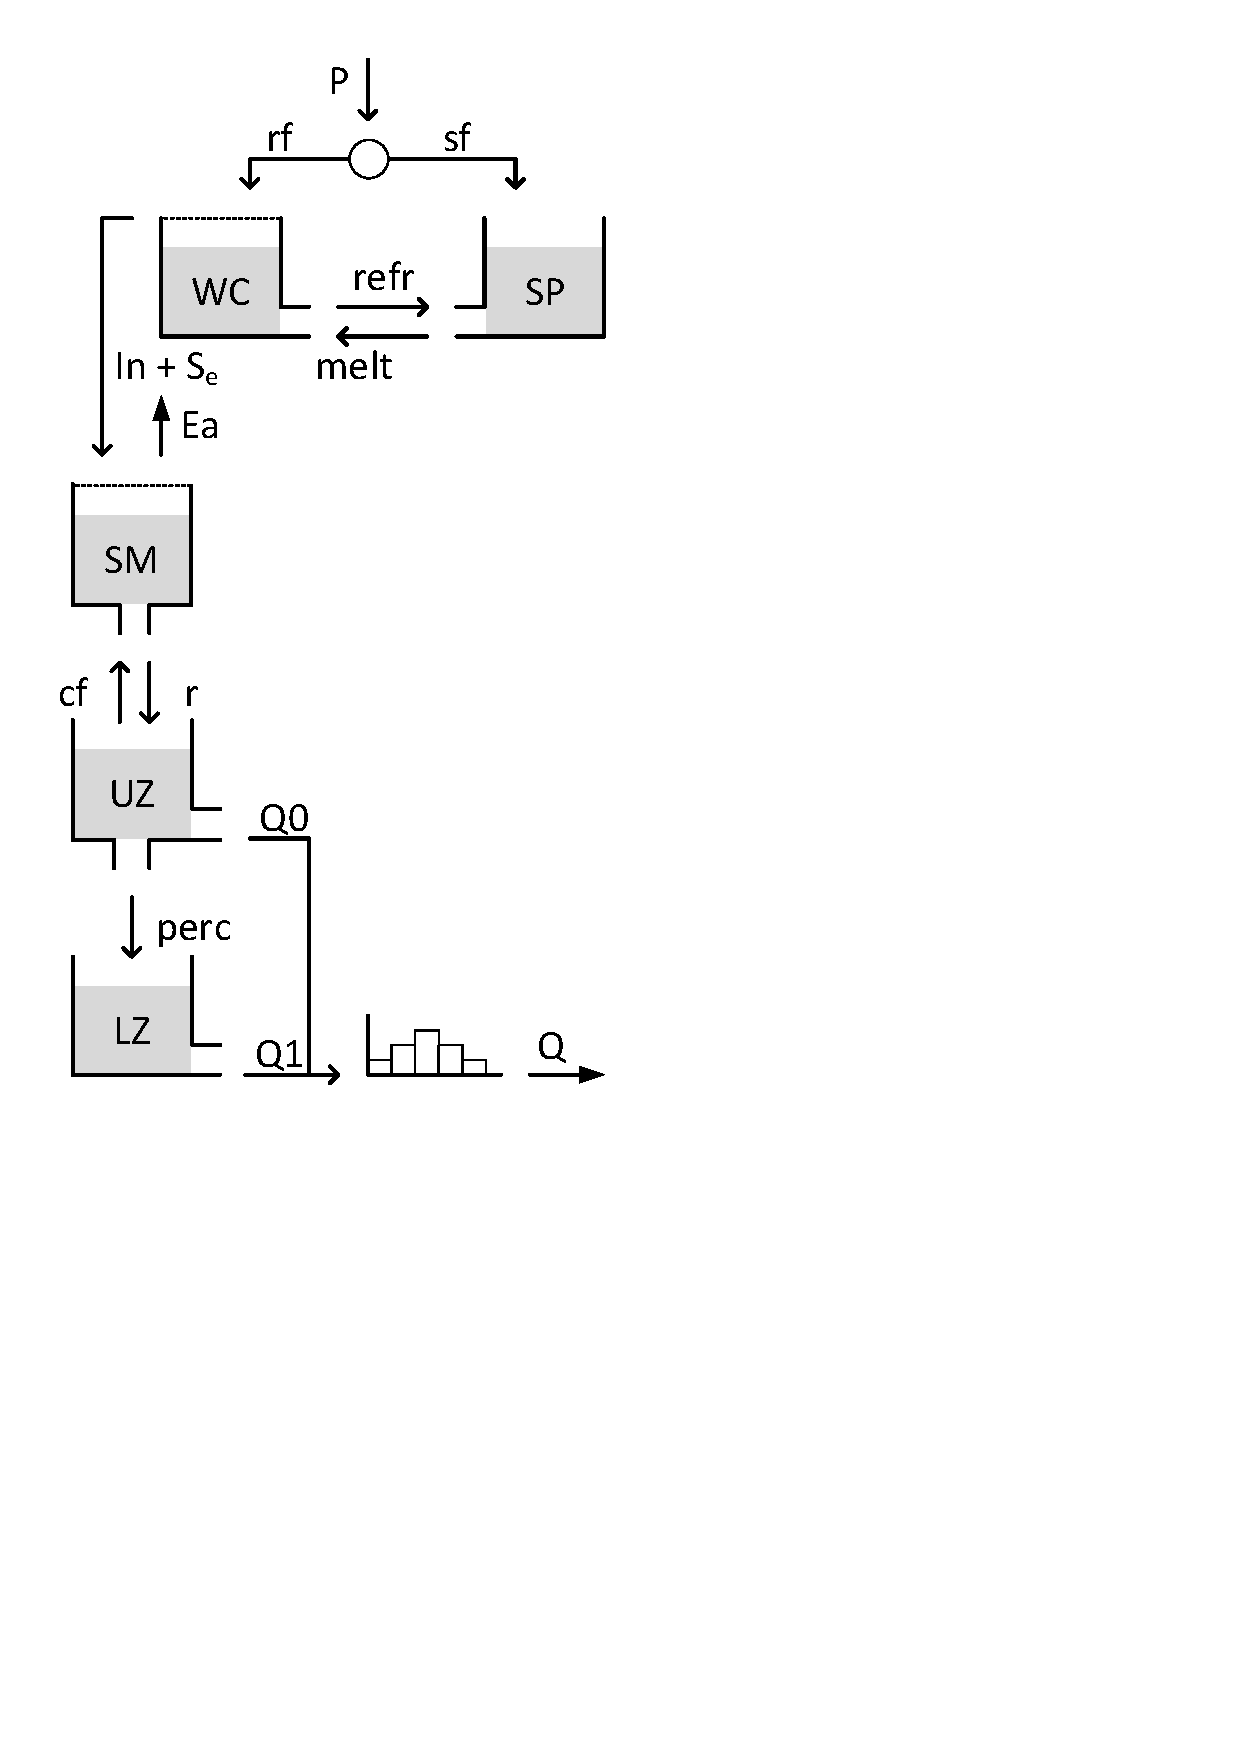
\includegraphics[trim=1cm 11.1cm 7cm 1cm,width=7cm,keepaspectratio]{./files/37_schematic.pdf}
\caption{Structure of the HBV-96 model} \label{fig:37_schematic}
\end{wrapfigure}

\begin{align}
	\frac{dSP}{dt} &= sf+refr-melt \\
	sf &= \begin{cases}
		P, &\text{if } T \leq TT-\frac{1}{2}TTI \\
		P*\frac{ TT+\frac{1}{2}TTI-T}{TTI}, &\text{otherwise}\\
		0, &\text{if } T \geq TT+\frac{1}{2}TTI \\
	\end{cases} \\
	refr &= 
	\begin{cases}
		CFR*CFMAX*(TTM-T), & \text{if } T < TTM \\
		0, & \text{otherwise}\\
	\end{cases}\\
	melt &= \begin{cases}
		CFMAX*(T-TTM), &\text{if } T \geq TTM\\
		0, &\text{otherwise}
	\end{cases}
\end{align}

Where SP is the current snow storage [mm]. $sf$ is precipitation that occurs as snowfall [mm/d] based on daily precipitation P [mm/d], threshold temperature for snowfall TT [\degree C] and the snowfall threshold interval length TTI [\degree C]. $refr$ [mm/d] is the refreezing of liquid snow if the current temperature T is below the melting threshold TTM [\degree C], using a coefficient of refreezing CFR [-] and a degree-day factor CFMAX [mm/d/\degree C]. $melt$ represents snowmelt if the current temperature T is below the melting threshold TTM, using the degree-day factor CFMAX. 

} % end of wrapfigure fix

\begin{align}
	\frac{dWC}{dt} &= rf+melt-refr-in-S_{excess}\\
	rf &= \begin{cases}
		0, &\text{if } T \leq TT-\frac{1}{2}TTI \\
		P*\frac{T- TT+\frac{1}{2}TTI}{TTI}, &\text{otherwise}\\
		P, &\text{if } T \geq TT+\frac{1}{2}TTI \\
	\end{cases} \\
	in &= \begin{cases}
		rf+melt, &\text{if } WC \geq WHC*SP\\
		0, &\text{otherwise}\\
	\end{cases}\\
	S_{e} &= \begin{cases}
		WC-WHC*SP, &\text{if } WC \geq WHC*SP\\
		0, &\text{otherwise}\\
	\end{cases}		
\end{align}

Where WC is the current liquid water content in the snow pack [mm], $rf$ is the precipitation occurring as rain [mm/d] based on temperature threshold parameters TT and TTI, $refr$ is the refreezing flux, and $in$ the infiltration to soil moisture [mm/d] that occurs when the water holding capacity of snow gets exceeded. $S_{excess}$ [mm/d] represents excess stored water that is freed when the total possible storage of liquid water in the snow pack is reduced.

\begin{align}
	\frac{dSM}{dt} &= (in+S_{excess})+cf-E_a-r\\
	cf &= CFLUX*\left(1-\frac{SM}{FC}\right)\\
	E_a &= \begin{cases}
		E_p, &\text{if } SM \geq LP*FC\\
		E_p*\frac{SM}{LP*FC}, &\text{otherwise}\\
	\end{cases}\\
	r &= (in+S_{excess})*\left(\frac{SM}{FC}\right)^\beta
\end{align}
  
Where SM is the current storage in soil moisture [mm], $in$ the infiltration from the surface, $cf$ the capillary rise [mm/d] from the unsaturated zone, $E_a$ evaporation [mm/d] and $r$ the flow to the upper zone [mm/d]. Capillary rise depends on the maximum rate CFLUX [mm/d], scaled by the available storage in soil moisture, expressed as the ration between current storage SM and maximum storage FC [mm]. Evaporation $E_a$ occurs at the potential rate $E_p$ when current soil moisture is above the wilting point LP [mm], and is scaled linearly below that. Runoff $r$ to the upper zone has a potentially non-linear relationship with infiltration in through parameter $\beta$ [-].

\begin{align}
	\frac{dUZ}{dt} &= r-cf-Q_0-perc \\
	Q_0 &= K_0*UZ^{(1+\alpha)}\\
	perc &= c.
\end{align}

Where UZ is the current storage [mm] in the upper zone. Outflow $Q_0$ [mm/d] from the reservoir has a non-linear relation with storage through time scale parameter $K_0$ [$d^{-1}$] and and $\alpha$ [-]. Percolation $perc$ [mm/d] to the lower zone is given as a constant rate $c$ [mm/d]S.

\begin{align}
	\frac{dLZ}{dt} &= perc-Q_1 \\
	Q_1 &= K_1*LZ
\end{align}

Where LZ is the current storage [mm] in the lower zone. Outflow $Q_1$ [mm/d] from the reservoir has a linear relation with storage through time scale parameter $K_1$ [$d^{-1}$]. Total outflow is generated by summing $Q_0$ and $Q_1$ and applying a triangular transform based on lag parameter MAXBAS [d].

\subsubsection{Parameter overview}
% Table generated by Excel2LaTeX from sheet 'Sheet1'
\begin{table}[htbp]
  \centering
    \begin{tabular}{lll}
    \toprule
    Parameter & Unit  & Description \\
    \midrule
    $TT$  & $^oC$ & Threshold temperature for snowfall \\
    $TTI$ & $^oC$ & Threshold temperature interval length \\
    $CFR$ & $-$   & Refreezing coefficient \\
    $CFMAX$ & $mm~^oC^{-1}~d^{-1}$ & Degree-day factor \\
    $TTM$ & $^oC$ & Threshold temperature for snowmelt \\
    $WHC$ & $-$   & Water holding capacity as fraction of current snow pack \\
    $CFLUX$ & $mm~d^{-1}$ & Maximum capillary rise rate \\
    $FC$  & $mm$  & Field capacity \\
    $LP$  & $-$   & Wilting point as fraction of $FC$ \\
    $\beta$ & $-$   & Recharge non-linearity \\
    $K_0$ & $d^{-1}$ & Runoff coefficient \\
    $\alpha$ & $-$   & Runoff non-linearity \\
    $c$   & $mm~d^{-1}$ & Percolation rate \\
    $K_1$ & $d^{-1}$ & Runoff coefficient \\
    $MAXBAS$ & $d$   & Unit Hydrograph time base \\
    \bottomrule
    \end{tabular}%
  \label{tab:addlabel}%
\end{table}%

